\section{Kontroler postaci (Bogna Lew)}\label{s:por_impl}
W trakcie rozgrywki istotnym aspektem wpływającym na jakość jest mechanizm sterowania postacią. Z tą mechaniką gracz ma
bezpośredni kontakt, ponieważ to właśnie za jej pomocą może eksplorować świat.

Do implementacji tego mechanizmu zainspirowaliśmy się grą Skyrim (por. \ref{s:walka}). Postać jest sterowana za pomocą klawiszy “W”, “A”, “S”
oraz “D”, natomiast jej rotacja oraz obrót kamery jest kontrolowany przez mysz. Dodatkowo gracz może wykonywać ataki
poprzez naciśnięcie lewego przycisku myszy.

Pierwszy element kontrolera odpowiada za przemieszczanie się postaci. Do tego wykorzystuje komponent \texttt{Input Manager}, w
którym zostały odwzorowane odpowiednie klawisze dla każdej z osi, wzdłuż której gracz może się przemieszczać. Na tej
podstawie wyznaczane jest faktyczne przesunięcie postaci względem kierunku, w którym jest zwrócona oraz modyfikowane
jest jej położenie. Dodatkowo ten komponent odpowiada za wyznaczenie prędkości, z jaką gracz się porusza. Domyślnie
postać przemieszcza się tempem chodu, jednakże jeśli gracz przytrzyma lewy klawisz Shift, to zacznie się poruszać biegiem.

Ten element dodatkowo odpowiada za wykrywanie, czy gracz chce wykonać atak. Przekazuje on następnie tę informację do
komponentu odpowiedzialnego za określenie powodzenia ataku oraz wywołanie odpowiedniego mechanizmu informowania
przeciwnika o odniesionych obrażeniach.

Druga część kontrolera odpowiada za ustawienie odpowiedniej animacji. Udostępnia metody umożliwiające uruchomienie
animacji ataków, odniesienia obrażeń, śmierci lub przemieszczania się. Ostatnia z nich wykorzystuje wartości zwrotu wzdłuż
obu osi oraz prędkość, które są wyznaczane w poprzednim komponencie. Na ich podstawie definiuje kolejne części nazwy
animacji, po czym, jeśli jest inna niż aktualnie wyświetlana, uruchamia ją.

Kolejny komponent nadzoruje rotację postaci oraz co za tym idzie - kamery. Analogicznie wykorzystywany jest \texttt{Input
Manager}, jednak w tym przypadku przechwytywane jest przesunięcie myszy. Komponent udostępnia graczowi możliwość
sterowania kierunkiem, w którym postać patrzy, a co za tym idzie - względem którego się przemieszcza. Jednocześnie
następuje dostosowanie położenia kamery tak, aby zawsze patrzyła w tym samym kierunku co postać gracza. Ponadto
komponent umożliwia zmianę wysokości oraz kąta patrzenia kamery. Dzięki temu gracz może dokładniej zobaczyć,
co znajduje się nad oraz tuż przed nim. Obrazują to rysunki \ref{fig:gora} oraz \ref{fig:dol}.

\begin{figure}[h!]
    \centering
    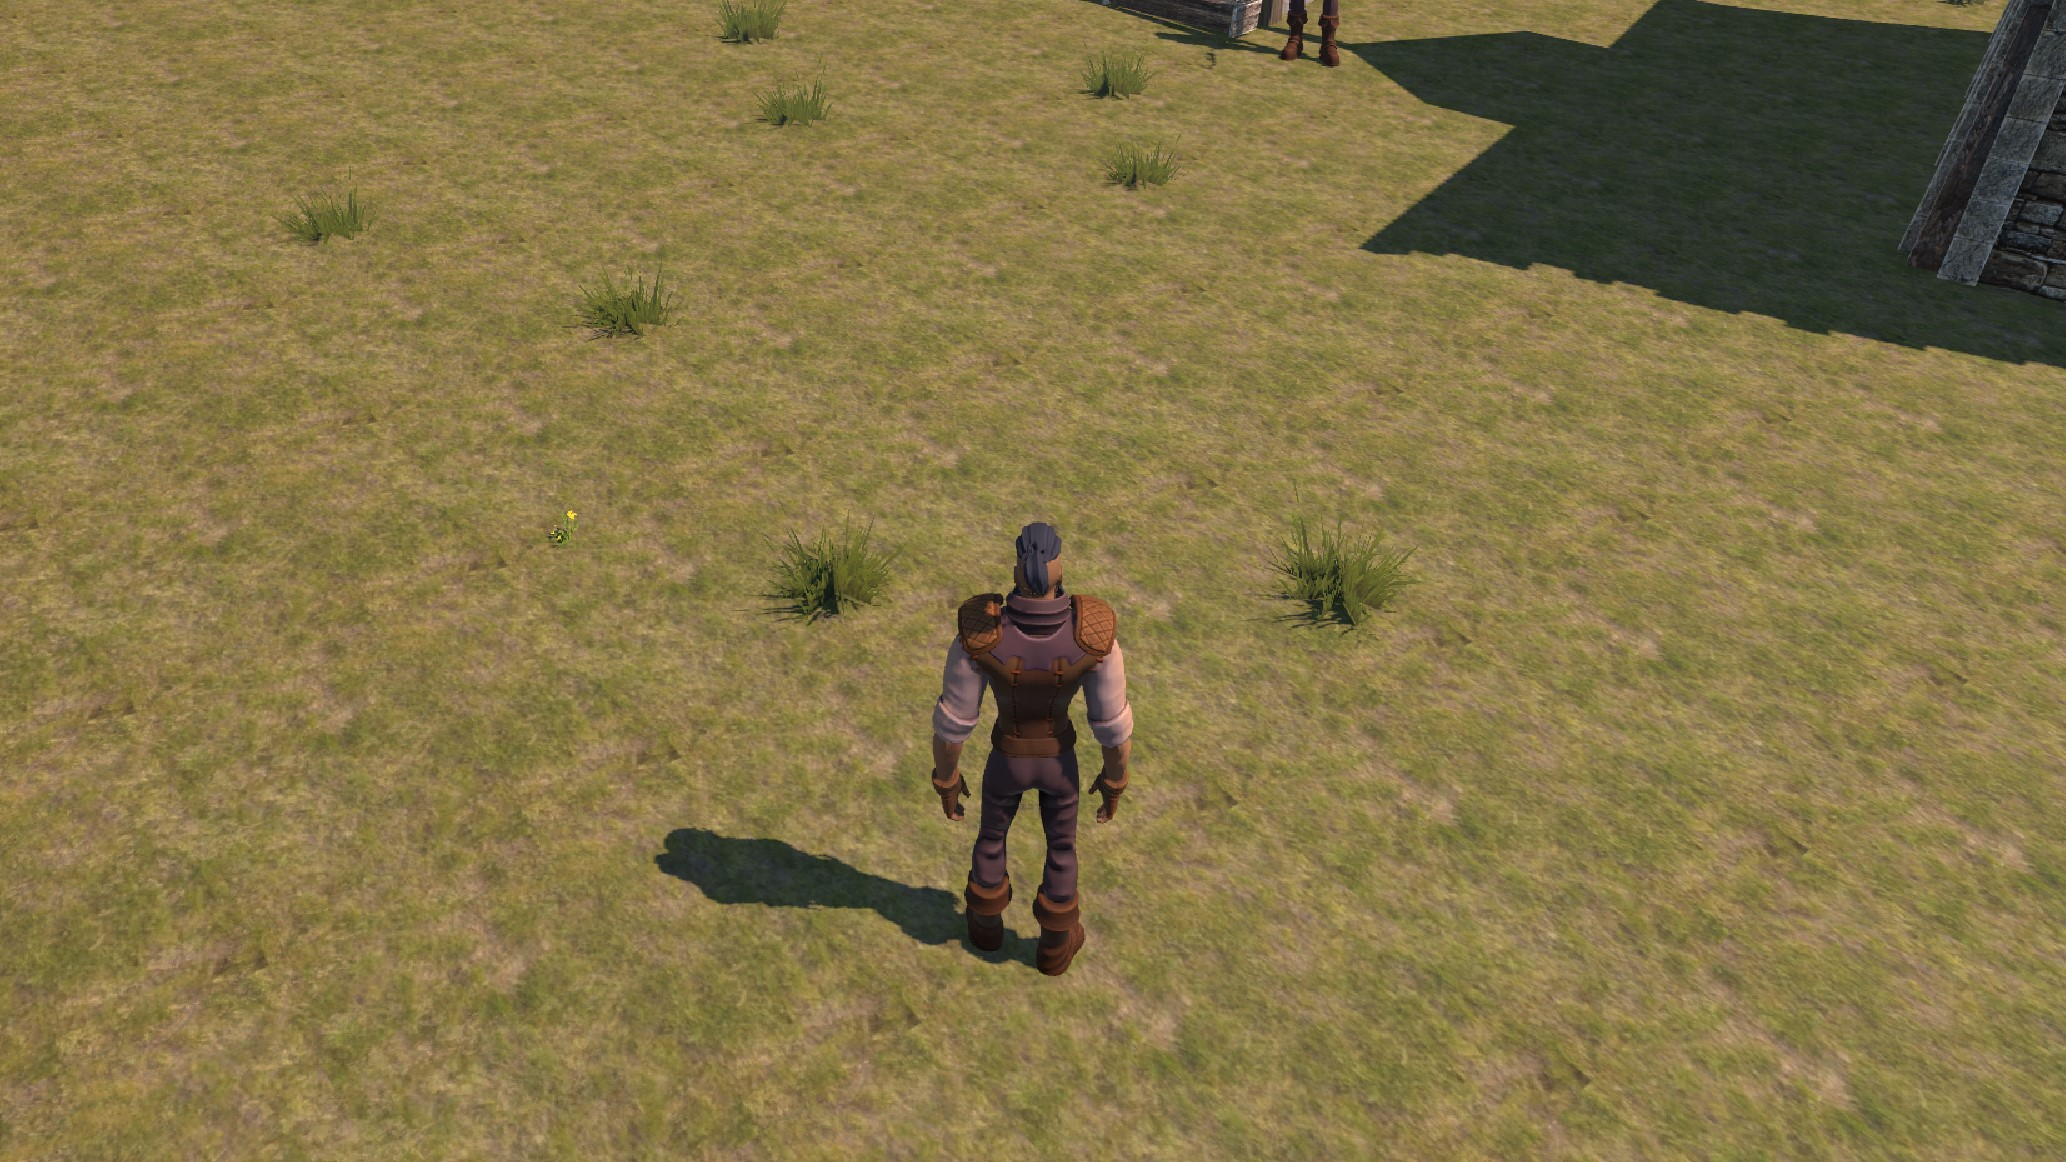
\includegraphics[width=0.9\textwidth]{images/implementacja/poruszanie_postacią/widok_z_gory.jpg}
    \caption{Widok po przesunięciu kamery w górę.}\label{fig:gora}
\end{figure}

\begin{figure}[h!]
    \centering
    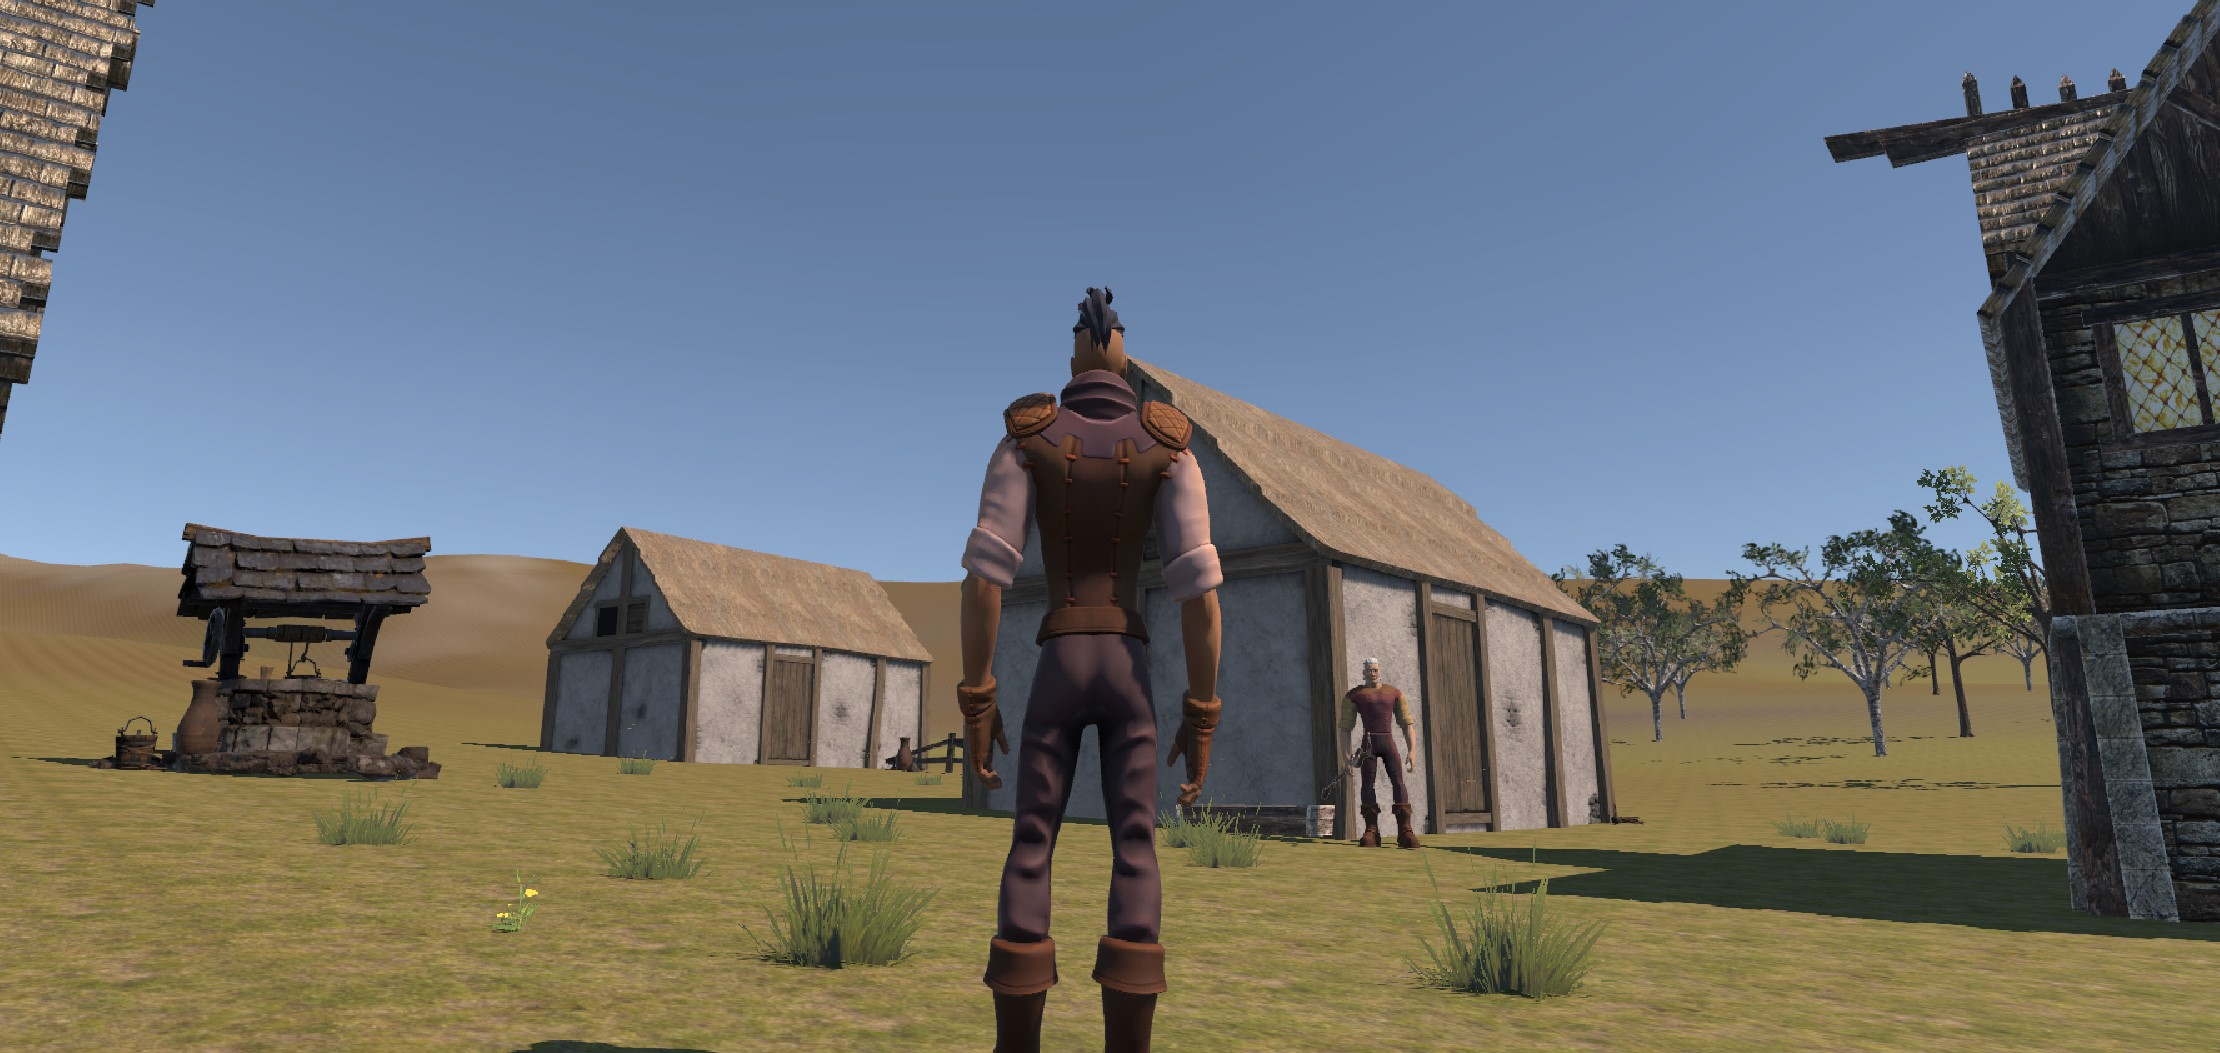
\includegraphics[width=0.9\textwidth]{images/implementacja/poruszanie_postacią/widok_z_dolu.jpg}
    \caption{Widok po przesunięciu kamery w dół.}\label{fig:dol}
\end{figure}

Ostatni komponent odpowiada za kontrolowanie przybliżania kamery. W tym celu w \texttt{Input Managerze} zostało odwzorowane kółko
myszy. Zwrócona przez system wartość jest wykorzystywana do obliczenia odległości kamery od postaci przy zachowaniu
ustalonych przez grę ograniczeń. Dodatkowo komponent dokonuje również automatycznego przybliżania, jeśli wskutek
przemieszczania się postaci, pomiędzy nią a kamerą miałaby się znaleźć przeszkoda. Dzięki temu nie zostanie zasłonięty
widok tego co się dzieje wokół postaci. Odsunięcie się od przeszkody zaskutkuje oddaleniem kamery do poprzedniej
odległości.
